\documentclass[UTF8]{article}


\usepackage[zihao=-4]{ctex} % ctex可以写中文,中括号里那句的意思是正文小四号
\usepackage[a4paper]{geometry} % 调整纸张大小和页边距的包,这里中括号中规定了纸张大小
\usepackage{array}
\usepackage{fancyhdr}
\usepackage{amsmath}
\usepackage{multirow}
\geometry{left=2.5cm,right=2.5cm,top=2.5cm,bottom=2.5cm} % 页边距设置
\usepackage{caption}
\usepackage{graphicx} % 用它在报告里加图
\graphicspath{{figures/}} % 指定图片所在文件夹
\pagestyle{fancy}
\rhead{用伸长法测定金属丝的杨氏模量}
\lhead{大学基础物理实验报告}
\cfoot{\thepage/6}
\rfoot{2023年 3月 3日}

\begin{document}
	\thispagestyle{empty}
	\vspace*{0.5cm}

	\begin{figure}[h]
		\centering
		
\includegraphics[width=0.7\linewidth]{logo}
	\end{figure}
\vspace*{0.1cm}
	\begin{center}
		\Huge{\textbf{大学基础物理实验报告}}\\
		\Huge{\textbf{《杨氏模量的测定》}}
		
		\vspace*{0.1cm}
	\end{center}
	\begin{table}[h]
		\centering	
		\begin{Large}
			\begin{tabular}{p{3cm} p{5cm}<{\centering}}
				姓\qquad 名: & xxx \\
				\hline
				学\qquad 院: & xxx \\
				\hline
				学\qquad 号: & xxxxxxx \\
				\hline
				分\qquad 组: & xxx \\
				\hline
				实验时间: & 2023.3.3\\
				\hline
				指导教师: & xxx\\
				\hline
			\end{tabular}
		\end{Large}
	\end{table}
	\clearpage
	\normalsize
		\begin{center}
		\LARGE\textbf{伸长法测量金属丝杨氏模量}
	\end{center}
	\subsection*{[实验目的要求]}
	\par 1.用伸长法测定金属丝的杨氏模量。
	\par 2.了解望远镜尺组的结构及使用方法。
	\par 3.掌握用光杠杆放大原理测量微小长度变化量的方法。
	\par 4.学习用对立影响法消除系统误差的思想方法。
	\par 5.学习用环差法处理数据。

	\subsection*{[实验仪器用具]}
	\par B款杨氏模量测定仪;螺旋测微器;游标卡尺;钢卷尺;
	\subsection*{[实验原理简述]}
	\subsubsection*{杨氏模量表达式}
	\par 金属丝长为$L$、截面积为S,在长度方向上施加作用力$F$使其伸长$\Delta L$\\
	 由胡克定律:
	 \begin{equation}
	 	\frac{F}{S}=E\frac{\Delta L}{L}
	 \end{equation}
	
	\par $(1)$式中$\dfrac{F}{S}$为\textbf{正应力},$\dfrac{\Delta L}{L}$为金属丝\textbf{相对伸长量},$E$为所求\textbf{杨氏模量}。\\
	即:
	\begin{equation*}
	E=\frac{FL}{S\Delta L}
	\end{equation*}
	\par 但金属的样式模量$E$通常很大,因此$\Delta L$十分微小难以测量,故需要用\textbf{放大法}的测量技术。若微小变化量用$\Delta L$表示放大后的测量值为$N$,则:
	\begin{equation*}
		A=\frac{N}{\Delta L}
	\end{equation*}
	\par $A$为放大器的\textbf{放大倍数},倍数越大,越有利于测量;倍数越小,信号失真量越小。本实验中所使用的A款杨氏模量测定仪使用的光杠杆属于光放大技术,对金属丝的长度进行了两次放大。此时$E$的表达式为
	\begin{equation}
		E=A\frac{FL}{SN}
	\end{equation}
	\clearpage
	\subsubsection*{B款杨氏模量测量仪}
		\begin{figure}[h]
			\centering
		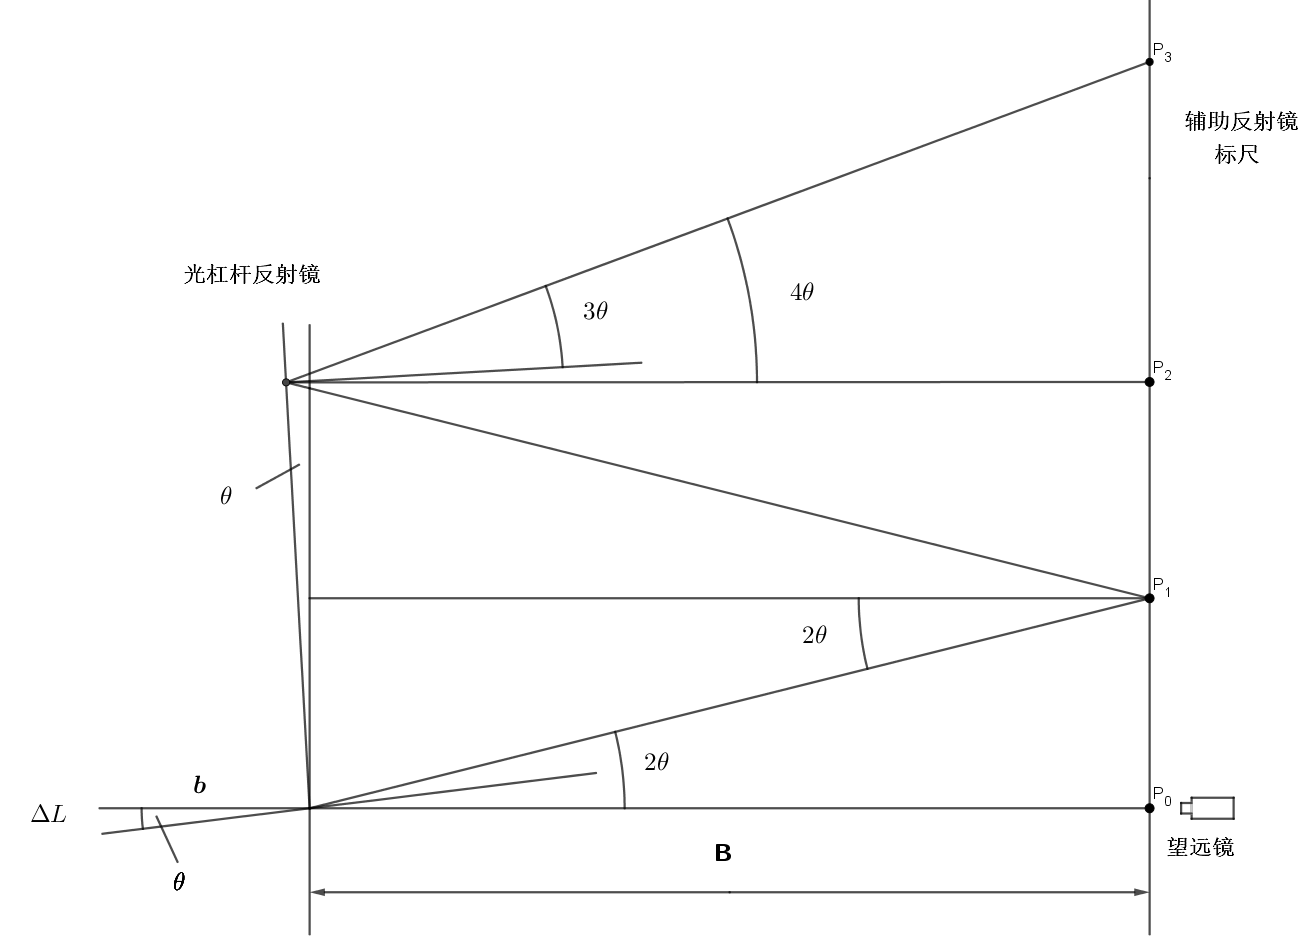
\includegraphics[width=0.7\linewidth]{picture2}
		\caption{光杠杆放大原理} %caption是图片的标题

		
	\end{figure}
	\par 图1为光杠杆的原理图,$B$为两平面镜的距离,$b$是光杠杆常量。当物体长度改变了$\Delta L$时,反射镜的角度改变了$\Delta\theta$,标尺光线经过光杠杆的两次反射和在辅助反射镜上的一次反射后到达标尺$P_3$处,放大后的钢丝伸长量即为$|P_3-P_0|$.,可知
	\[\Delta h = |P_3-P_0| = Btan4\theta+Btan2\theta+Btan2\theta\]

	\par 当$\theta\to0$时,可作近似$tan\theta\approx\theta=\dfrac{\Delta L}{b}$,带入则有
	\[\Delta L = \dfrac{b\Delta h}{8B}\]
	\par 
	\par 其中$\dfrac{8B}{b}$为放大倍数,注意:等式成立的条件为:$\theta\to0$将上述式子带入$(2)$式,并利用$S=\pi R^2$和$F = mg$,可得$E$的测量结果为
	\begin{equation}
		E=\frac{32BLmg}{\pi D^2b\Delta h}
	\end{equation}
	\subsection*{[实验步骤]}
	\par 1.将望远镜尺组移动到靠近平面镜的地方,调节望远镜尺组的高度与平面镜等高;移动望远镜尺组,使标尺距平面镜略大于最短视距
	\par 2.打开灯光,调节平面镜的仰角和标尺高度,使得能在望远镜上方看到标尺的一大一小两个相且望远镜内能看到较小的;调节望远镜的内调焦手轮使成像清晰,记录下分划板准线对应的标尺刻度的初始数值。
	\par 3.按等时间间隔(两分钟)递加一个砝码。记录下相应读数;等到砝码加完后再按等时间间隔递减一个砝码,再次记录下相应读数。 保持伸长仪和光杆杆不动,用卷尺测量出平面镜间距和金属丝长度;用螺旋测微器在金属丝三个不同位置测量两次直径;将光杠杆放在平纸上,轻印三足之痕迹,然后用游标卡尺测量痕迹间距离。
	\subsection*{[数据处理]}
	

\subsubsection*{处理$B$,$L$,$b$}
\begin{table}[h]
	\centering
	\begin{tabular}{|l|l|l|l|}
		\hline
		平面镜间距$B$ & 金属丝原长$L$ & 光杠杆常量$b$ &      \\ \hline
		91     & 37.6   & 4.48  & 单位:cm \\ \hline
	\end{tabular}
	\caption{$B$,$L$,$b$的测量值}
\end{table}
\[\mu_{b}=0.02mm \quad\mu_L = \frac{0.5}{3}mm \quad\mu_B = \frac{0.5}{3}mm\]
\subsubsection*{处理伸长量$\Delta$ L}

\begin{table}[h]
	
	\centering
	\begin{tabular}{|l|l|lll|ll|}
		\hline
		\multirow{2}{*}{次数} & \multirow{2}{*}{拉力示值/kg} & \multicolumn{3}{l|}{标尺读数/cm}                                  & \multicolumn{2}{l|}{环差法}                                               \\ \cline{3-7} 
		&                          & \multicolumn{1}{l|}{加载}   & \multicolumn{1}{l|}{减载}   & 平均    & \multicolumn{1}{l|}{}                       & 平均                       \\ \hline
		1                   & 0.1                       & \multicolumn{1}{l|}{5.1}  & \multicolumn{1}{l|}{5.15} & 5.125 & \multicolumn{1}{l|}{\multirow{2}{*}{2.6}}   & \multirow{8}{*}{2.63125} \\ \cline{1-5}
		2                   & 0.2                      & \multicolumn{1}{l|}{5.75} & \multicolumn{1}{l|}{5.8}  & 5.775 & \multicolumn{1}{l|}{}                       &                          \\ \cline{1-6}
		3                   & 0.3                        & \multicolumn{1}{l|}{6.35} & \multicolumn{1}{l|}{6.45} & 6.4   & \multicolumn{1}{l|}{\multirow{2}{*}{2.625}} &                          \\ \cline{1-5}
		4                   & 0.4                        & \multicolumn{1}{l|}{7.05} & \multicolumn{1}{l|}{7.1}  & 7.075 & \multicolumn{1}{l|}{}                       &                          \\ \cline{1-6}
		5                   & 0.5                        & \multicolumn{1}{l|}{7.7}  & \multicolumn{1}{l|}{7.75} & 7.725 & \multicolumn{1}{l|}{\multirow{2}{*}{2.65}}  &                          \\ \cline{1-5}
		6                   & 0.6                      & \multicolumn{1}{l|}{8.35} & \multicolumn{1}{l|}{8.45} & 8.4   & \multicolumn{1}{l|}{}                       &                          \\ \cline{1-6}
		7                   & 0.7                        & \multicolumn{1}{l|}{9.05} & \multicolumn{1}{l|}{9.05} & 9.05  & \multicolumn{1}{l|}{\multirow{2}{*}{2.65}}  &                          \\ \cline{1-5}
		8                   & 0.8                      & \multicolumn{1}{l|}{9.75} & \multicolumn{1}{l|}{9.7}  & 9.725 & \multicolumn{1}{l|}{}                       &     \\ \hline
	\end{tabular}
	\caption{$\Delta h$的测量值}
\end{table}\par 通过$\Delta L = \dfrac{b\Delta h}{8B}$,可得到
\begin{table}[h]
\centering
\begin{tabular}{|l|l|l|l|l|l|}
	\hline
	& 1     & 2        & 3        & 4        & 均值       \\ \hline
	$\Delta L$计算值/cm & 0.016 & 0.016154 & 0.016308 & 0.016308 & 0.016192 \\ \hline
\end{tabular}
\caption{$\Delta L$的计算值}
\end{table}
\par 1.$\Delta L$的$A$类不确定度$\mu_{a\Delta L}$公式为
\[ \mu_{a\Delta L}=t_{(0.683,3)}\cdot\frac{\sqrt{\sum_{i=1}^{n=6}(\Delta L_i-\overline{\Delta L})^2}}{\sqrt{n}\cdot\sqrt{n-1}}=t_{(0.683,3)}\cdot\frac{\sqrt{6(\overline{\Delta L_i^2}-\overline{\Delta L }^2)}}{\sqrt{n}\cdot\sqrt{n-1}}\]
\clearpage
\par 带入$\overline{\Delta L}=0,016192$,\quad$t_{(0.683,3)}=1.20$后计算得到:

\begin{align*}
	\mu_{a\Delta L}&=1.20\cdot \frac{\sqrt{0.016000^2+0.016154^2+2\times0.016308^2-4\times0.016192^2}}{\sqrt{4}\cdot\sqrt{3}}\\
	&=1.2489\times10^{-4}  \quad (cm)     
\end{align*}
\par 2.$\Delta L$的$B$类不确定度为$\mu_{b\Delta L}=\dfrac{0.01}{\sqrt{3}}cm$,从而合成$\Delta L$的不确定度:
\[\mu_{\Delta L}=\sqrt{\mu_{a\Delta L}^2+\mu_{b\Delta L}^2}=\sqrt{1,2489^2\times 10^{-8}+\frac{10^{-4}}{3}}\approx 0.0058\quad(cm)\]

\subsubsection*{处理金属丝直径$D$}

\begin{table}[h]
	\centering
	\begin{tabular}{|l|l|l|l|l|l|l|l|}
	\hline
	测量次数 & 1     & 2     & 3     & 4     & 5     & 6     & 平均值$\overline{D}$      \\ \hline
	D/mm & 0.799 & 0.802 & 0.802 & 0.801 & 0.799 & 0.798 & 0.8001 \\ \hline
	\end{tabular}
\caption{金属丝直径$D$的测量值}
\end{table}
\par 1.$D$的$A$类不确定度$\mu_{aD}$公式为
\[ \mu_{aD}=t_{(0.683,5)}\cdot\frac{\sqrt{\sum_{i=1}^{n=6}(D_i-\overline{D})^2}}{\sqrt{n}\cdot\sqrt{n-1}}=t_{(0.683,5)}\cdot\frac{\sqrt{6(\overline{D_i^2}-\overline{D}^2)}}{\sqrt{n}\cdot\sqrt{n-1}}\]
\par 带入$\overline{D}=0,800$,\quad$t_{(0.683,5)}=1.11$后计算得到:
\begin{align*}
	\mu_{aD}&=1.11\cdot \frac{\sqrt{0.799^2+2\times0.802^2+0.801^2+0.799^2+0.798^2-6\times0.800^2}}{\sqrt{6}\cdot\sqrt{5}}\\
		&=0.0081\quad (mm)
\end{align*}
\par 2.$D$的$B$类不确定度$\mu_{bD}=\dfrac{0.001}{\sqrt{3}}mm$,从而合成
\begin{align*}
	\mu_D &= \sqrt{\mu_{aD}^2+\mu_{bD}^2} = \sqrt{0.0081^2+\left(\frac{0.001}{\sqrt{3}}\right)^2} = 0.0082 \quad (mm)
\end{align*}
\subsubsection*{$E$的不确定度}
\[E=\frac{32mgBL}{\pi bD^2\Delta L}\]
\par 带入数据后:
\clearpage
\[\overline{E} = \frac{32\times4\times9.8N\times0.91m\times0.376m}{\pi\times0.0448m\times0.0008^2m^2\times0.00016192m}\approx2.94\times10^{13}\]
$E$的不确定度公式为:
\[	\mu_E = \overline{E}\cdot\sqrt{\left(\frac{\mu_{\Delta L}}{\Delta \overline{L} }\right)^2+\left(\frac{2\mu_{D}}{\overline{D} }\right)^2+\left(\frac{\mu_{B }}{\overline{B} }\right)^2+\left(\frac{\mu_{b}}{\overline{b} }\right)^2+\left(\frac{\mu_{L}}{\overline{L} }\right)^2}\\\]
\begin{align*}
	&=\overline{E}\cdot\sqrt{\left(\frac{0.0058}{0.016192}\right)^2+\left(\frac{2\times0.0082}{0.8001}\right)^2+\left(\frac{0.002}{4.48}\right)^2+\left(\frac{0.05}{3\times91}\right)^2+\left(\frac{0.05}{3\times37.6}\right)^2}\\
	&\approx1.055\times10^{13}
\end{align*}
\par 故$E$的值为
\[E = (2.9\pm1.0)\times10^{13}\quad (N/m^2)\] 
\subsubsection*{误差分析}
\par 只需找出对$E$的不确定度影响最大的因素,从$\mu_E$的具体计算式来看,$u_{\Delta  L}$的$B$类不确定度通过影响了$\mu_L$从而影响了最后的结果,故本实验主要误差来自于伸长量的$B$类不确定度。
\subsection*{[思考题]}
\par 1.$\Delta L$和$D$的测量误差较大,本实验中通过光杠杆放大法将$\Delta L$放大为$\Delta h$进行测量,并且通过加载砝码和减载砝码的方式使用对立影响法消除和减弱金属丝弹性滞后效应的影响,并在处理数据的时候使用了环差法。对于$D$本实验在金属丝的三个不同位置测量最后取平均值。
\par 2.可以通过适量增大$B$或者减小$b$的方式来提高放大倍数。这样做可以使得读数更加精准,但是有可能会放大实验的系统误差,且增大的$B$不能超过望远镜的最大视距,减小的$b$也应该保证实验的可行性。
\par 3.略前倾好。因为金属丝的微小形变一定程度上会改变平面镜的倾角,开始就向前倾可以减少这一因素的影响,属于对立影响法。假定初始位置时,反射镜面与铅锤面成$5^o$向后仰,会给实验带来很大误差。
\end{document}